\documentclass[11pt,a4paper]{article}
\usepackage[utf8]{inputenc}
\usepackage[spanish]{babel}	%Idioma
\usepackage{amsmath}
\usepackage{amsfonts}
\usepackage{amssymb}
\usepackage{graphicx} 	%Añadir imágenes
\usepackage{geometry}	%Ajustar márgenes
\usepackage[export]{adjustbox}[2011/08/13]
\usepackage{float}
\restylefloat{table}
\usepackage{diagbox}
\usepackage{makecell}
\usepackage[hidelinks]{hyperref}
\usepackage{titling}
%\graphicspath{{/home/nazaret/Escritorio/LaTEX}}
%\usepackage{minted}
\usepackage{multirow}
\usepackage{caption}
\usepackage{multicol}
\usepackage{array}
\selectlanguage{spanish}
\usepackage{xcolor}

%Opciones de encabezado y pie de página:
\usepackage{fancyhdr}
\pagestyle{fancy}
\lhead{Nazaret Román Guerrero}
\rhead{Sistemas Multimedia}
\lfoot{Grado en Ingeniería Informática}
\cfoot{}
\rfoot{\thepage}
\renewcommand{\headrulewidth}{0.4pt}
\renewcommand{\footrulewidth}{0.4pt}

%Opciones de fuente:
\usepackage[utf8]{inputenc}
\usepackage[default]{sourcesanspro}
\usepackage{sourcecodepro}
\usepackage[T1]{fontenc}

\setlength{\parindent}{15pt}
\setlength{\headheight}{15pt}
\setlength{\voffset}{10mm}

% Custom colors
\usepackage{color}
\definecolor{deepblue}{rgb}{0,0,0.5}
\definecolor{deepred}{rgb}{0.6,0,0}
\definecolor{deepgreen}{rgb}{0,0.5,0}

\usepackage{listings}

\begin{document}
\begin{titlepage}

\begin{minipage}{\textwidth}

\centering

\includegraphics[width=0.5\textwidth]{logo.png}\\

\textsc{\Large Sistemas Multimedia\\[0.2cm]}
\textsc{GRADO EN INGENIERÍA INFORMÁTICA}\\[1cm]

{\Huge\bfseries Imagen\\}
\noindent\rule[-1ex]{\textwidth}{3pt}\\[3.5ex]
{\large\bfseries Trabajo voluntario}
\end{minipage}

\vspace{1.5cm}
\begin{minipage}{\textwidth}
\centering

\textbf{Autora}\\ {Nazaret Román Guerrero}\\[2.5ex]

\includegraphics[width=0.3\textwidth]{etsiit.jpeg}\\[0.1cm]
\vspace{1cm}
\textsc{Escuela Técnica Superior de Ingenierías Informática y de Telecomunicación}\\
\vspace{1cm}
\textsc{Curso 2018-2019}
\end{minipage}
\end{titlepage}

\pagenumbering{gobble}
\pagenumbering{arabic}
\tableofcontents
\thispagestyle{empty}

\newpage

\section{Parámetros}

Vamos a comparar distintas imágenes, 7 imágenes concretamente. Para ello, utilizaremos diferentes \textit{códecs}, y, en el caso de que éste lo permita, variaremos algunos parámetros como la compresión. Usaremos las siguientes imágenes, todas en formatos sin compresión (\textsc{.dng} las 4 primeras, \textsc{.bmp} las 3 últimas).

\begin{enumerate}
	\item Imagen con pocos colores (\textsc{poco\_crom.dng}).
	\item Imagen con mucha riqueda cromática (\textsc{crom.dng}).
	\item Imagen de una persona (\textsc{retrato.dng}).
	\item Imagen con pocas texturas (\textsc{pocas\_texturas.dng}).
	\item Imagen con muchas texturas (\textsc{texturas.bmp}).
	\item Imagen con texto (\textsc{texto.bmp}).
	\item Imagen gráfica (\textsc{graficos.bmp}).
\end{enumerate}

Para cada imagen, crearemos una tabla con cada \textit{códec} en una fila y tres columnas indicando el tamaño de la imagen, la valoración que se le da, y la posición en el ranking. Para la valoración se utilizarán iconos, descritos más abajo.\\

Además, para los \textsc{códecs} que admitan compresión, habrá más filas correspondientes a dicha compresión. Para las imágenes en \textsc{jpeg}, para hablar de compresión hablaremos de ``calidad'', un valor que estará entre 1 y 100 (donde 1 es máxima compresión y peor calidad, y 100 es máxima calidad pero nada de compresión). Para las imágenes en \textsc{tiff} simplemente hablaremos de compresión, y será uno de entre los dos siguientes: sin compresión o compresión con deflación.\\

Los iconos que se van a utilizar para las valoraciones son:

\begin{itemize}
	\item Muy buena = 
\includegraphics[width=0.05\textwidth]{mb.png}
	\item Buena = 
\includegraphics[width=0.05\textwidth]{b.png}
	\item Regular = 
\includegraphics[width=0.05\textwidth]{r.png}
	\item Mala = 
\includegraphics[width=0.05\textwidth]{m.png}
	\item Muy mala = 
\includegraphics[width=0.05\textwidth]{mm.png}
\end{itemize}


\subsection{Imagen con pocos colores}

Esta primera imagen, mostrada debajo, utilizaremos una imagen tomada de un manga, los cuales son impresos en escala de grises.

\begin{itemize}
	\item Formato original: \textsc{.dng}
	\item Tipo de imagen: poco cromática
	\item Imagen:
		\begin{figure}[H]
		\centering
			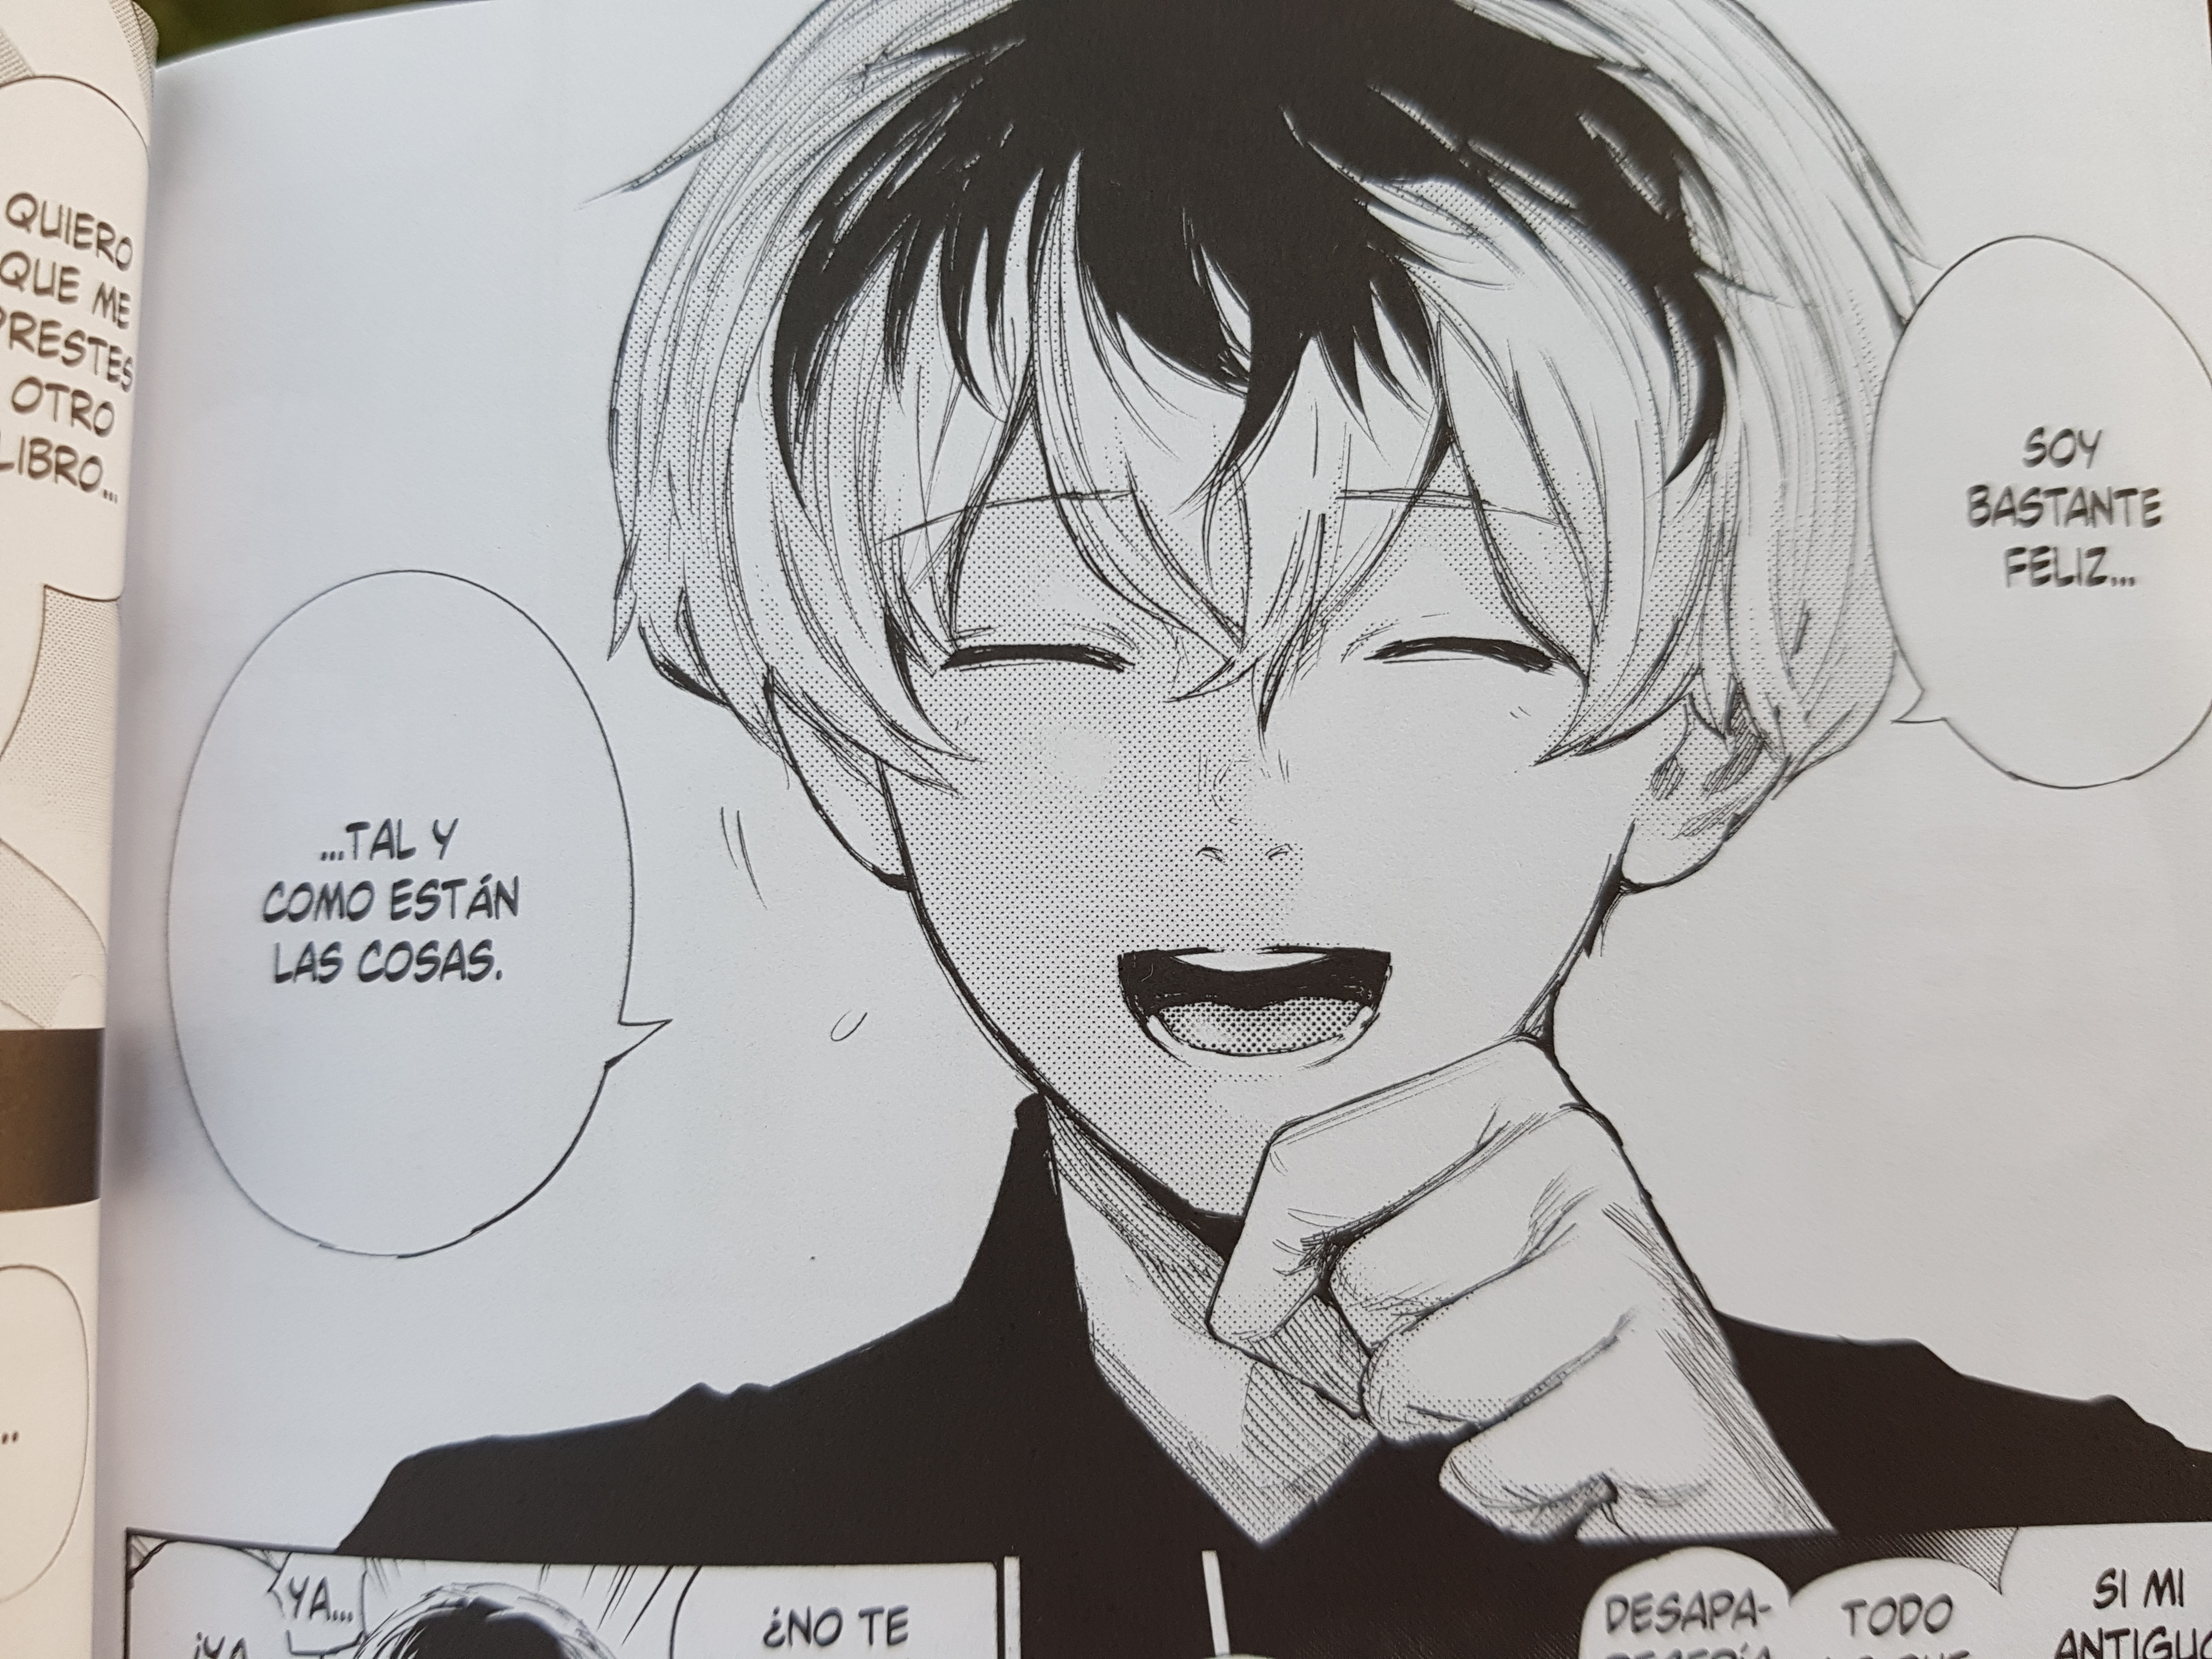
\includegraphics[width=0.5\textwidth]{Fotos/poco_crom.jpg}
		\end{figure}	
\end{itemize}

\begin{table}[H]
\centering
\begin{tabular}{|c|c|c|c|}
\hline
\diagbox[width=15em]{\textit{Códec}/Formato}{\\Información} & Tamaño & Valoración & Ranking \\
\hline
\textsc{bmp} & 36.4 MB & 
\includegraphics[width=0.03\textwidth]{mb.png} & 1º \\ \hline
\textsc{tiff} sin compresión & 36.6 MB & 
\includegraphics[width=0.03\textwidth]{b.png} & 2º \\ \hline
\textsc{tiff} con deflación & 29.2 MB & 
\includegraphics[width=0.03\textwidth]{b.png} & 2º \\ \hline
\textsc{gif} & 9.7 MB & 
\includegraphics[width=0.03\textwidth]{mb.png} & 1º \\ \hline
\textsc{jpeg} con calidad :100 & 17.3 MB & 
\includegraphics[width=0.03\textwidth]{b.png} &  2º \\ \hline
\textsc{jpeg} con calidad :50 & 731.9 kB & 
\includegraphics[width=0.03\textwidth]{b.png} &  2º \\ \hline
\textsc{jpeg} con calidad :5 & 144 kB & 
\includegraphics[width=0.03\textwidth]{mm.png} & 3º \\ \hline
\textsc{png} & 22.4 MB & 
\includegraphics[width=0.03\textwidth]{b.png} & 2º \\ \hline
\end{tabular}
\caption{Imagen poco cromática}
\label{tab:my-table}
\end{table}

\newpage

\subsubsection{Conclusión}

En esta imagen del manga de \textit{Tokyo Ghoul:re}, en escala de grises, aquellos \textit{códecs} que permiten menos profundidad de color, es decir, que tienen menos variedad de color (y por tanto menos tonos de gris), hace que los colores se marquen mejor ya que la finalidad de un manga es que se vea en blanco o negro. Por tanto, se aprecian mejor estos colores en \textsc{.gif} y \textsc{.bmp}

\subsection{Imagen con muchos colores}

Esta primera imagen, mostrada debajo, utilizaremos una imagen tomada de un manga, los cuales son impresos en escala de grises.

\begin{itemize}
	\item Formato original: \textsc{.dng}
	\item Tipo de imagen: muy cromática
	\item Imagen:
		\begin{figure}[H]
		\centering
			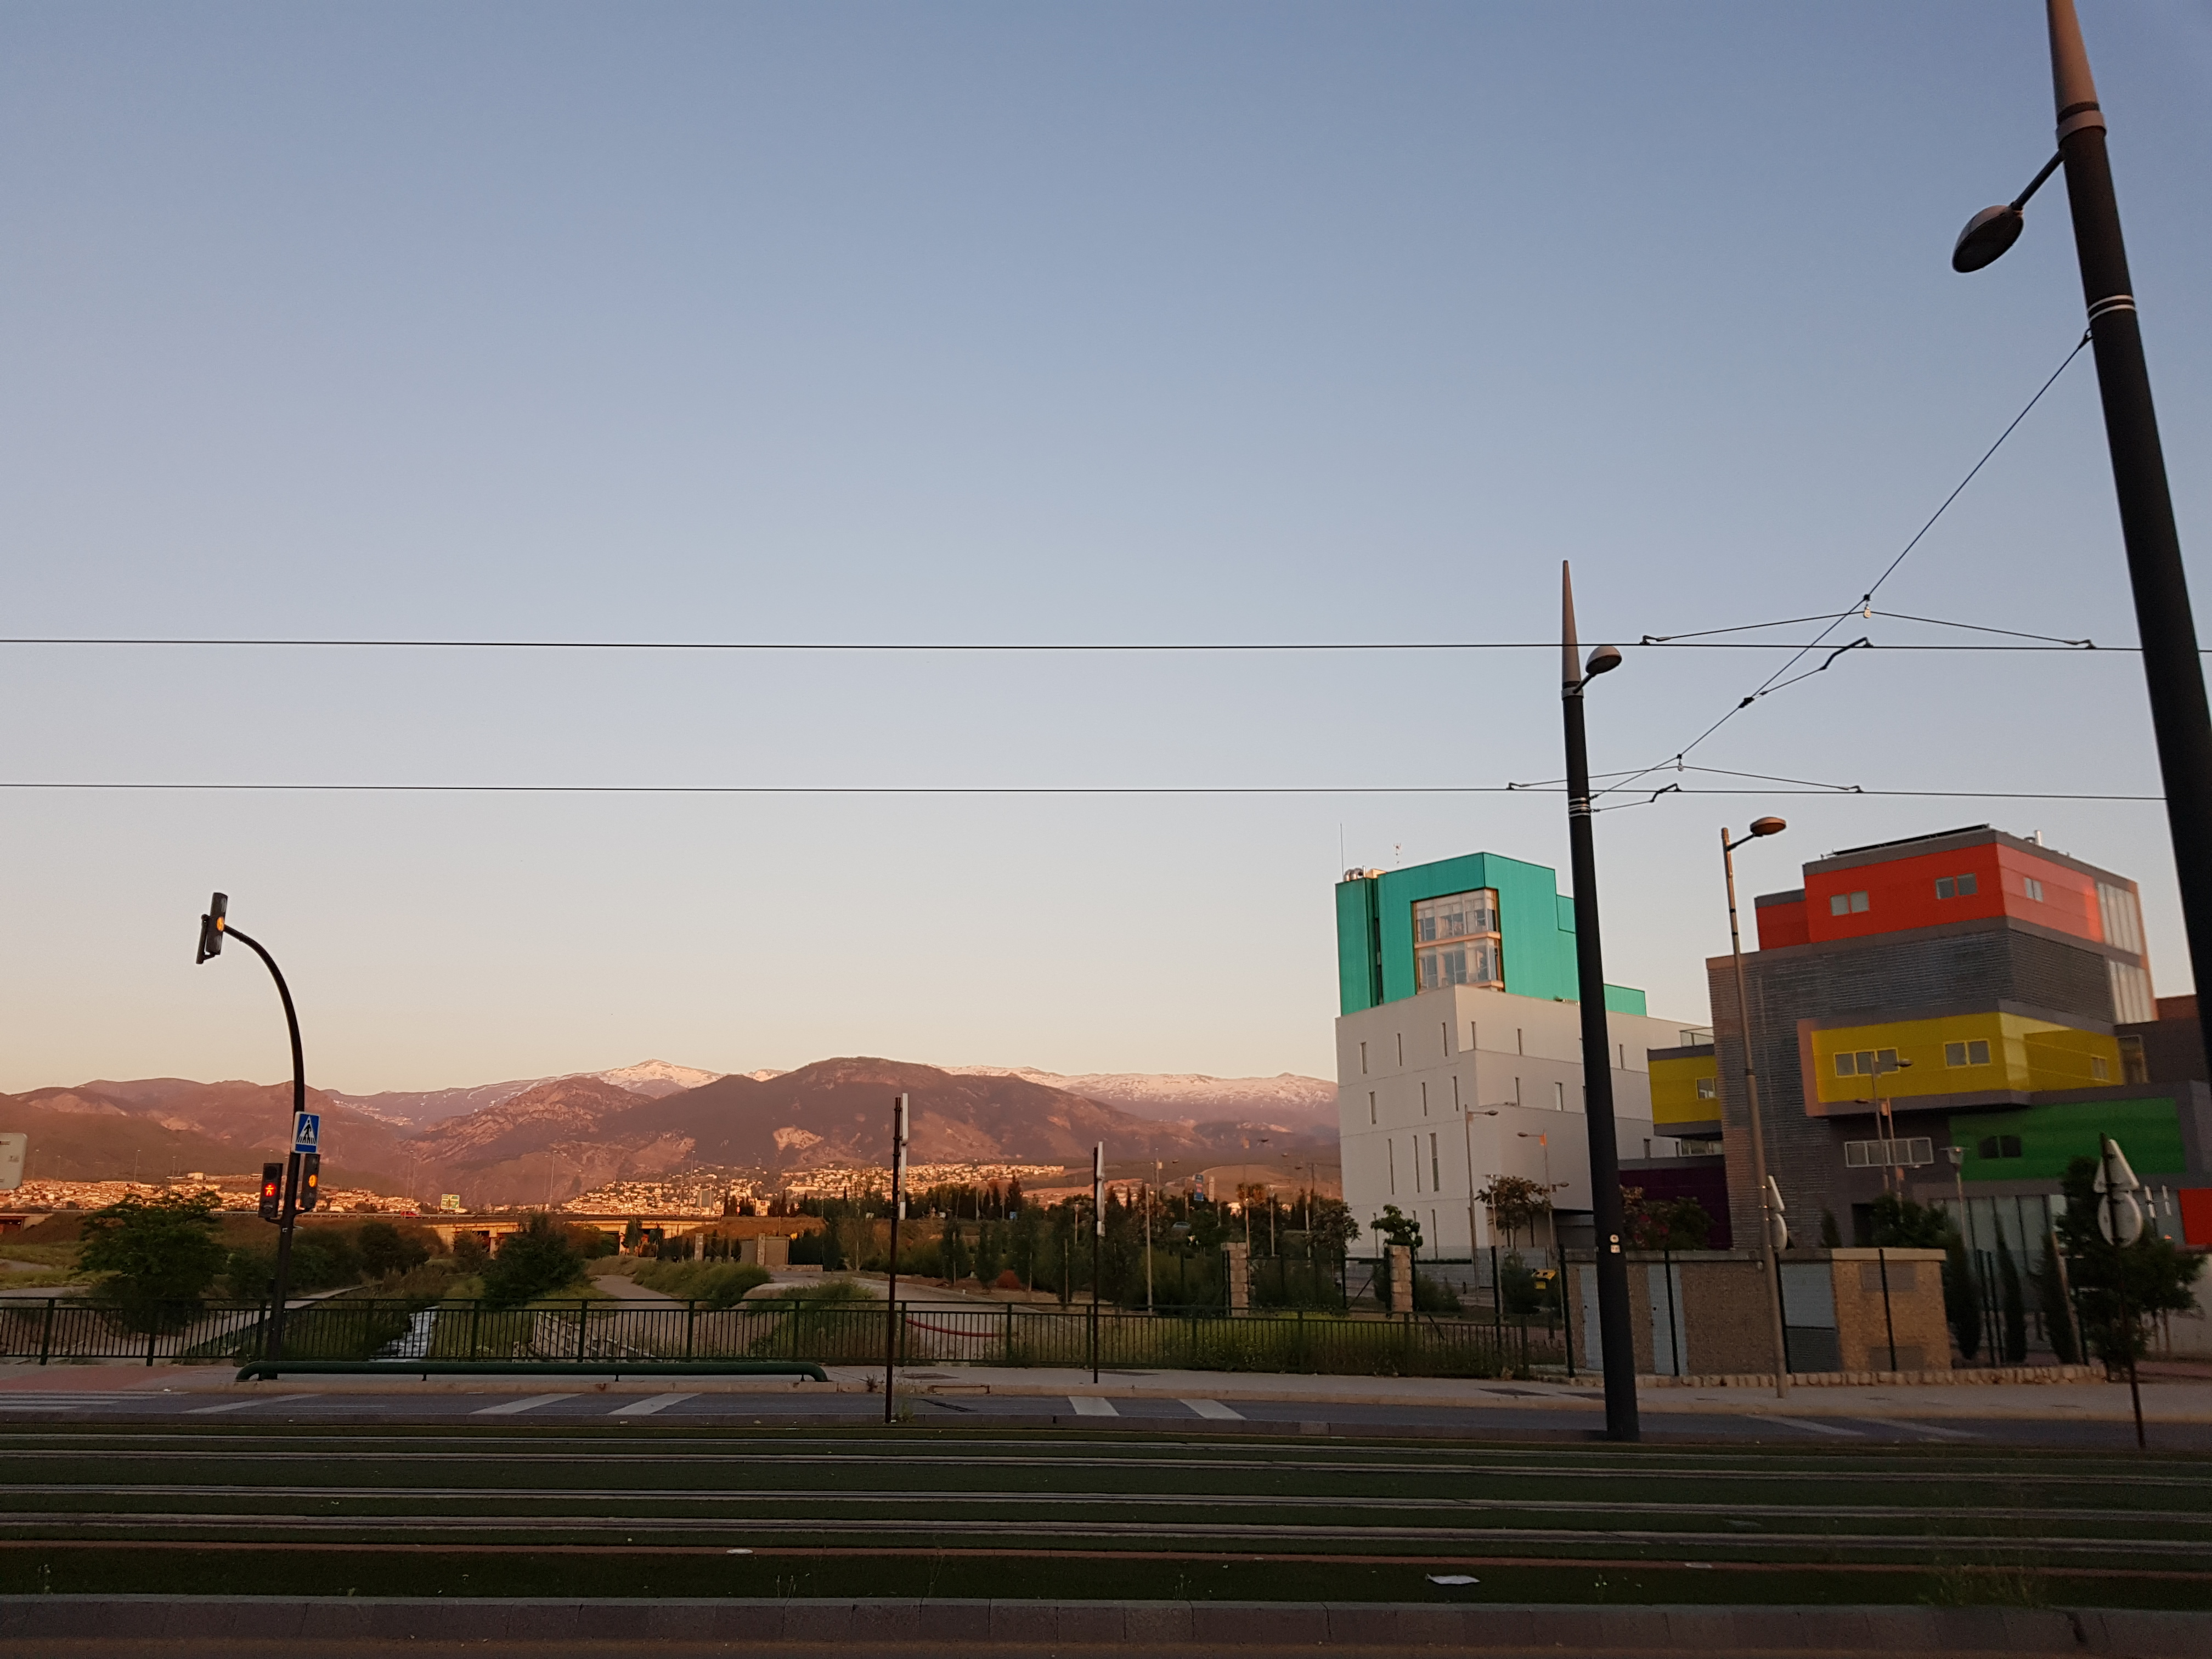
\includegraphics[width=0.5\textwidth]{Fotos/crom.jpg}
		\end{figure}	
\end{itemize}

\begin{table}[H]
\centering
\begin{tabular}{|c|c|c|c|}
\hline
\diagbox[width=15em]{\textit{Códec}/Formato}{\\Información} & Tamaño & Valoración & Ranking \\
\hline
\textsc{bmp} &  &  &  \\ \hline
\textsc{tiff} sin compresión &  &  &  \\ \hline
\textsc{tiff} con deflación &  &  &  \\ \hline
\textsc{gif} &  &  &  \\ \hline
\textsc{jpeg} con calidad :100 &  &  &  \\ \hline
\textsc{jpeg} con calidad :50 &  &  &  \\ \hline
\textsc{jpeg} con calidad :5 &  &  &  \\ \hline
\textsc{png} &  &  &  \\ \hline
\end{tabular}
\caption{Imagen poco cromática}
\label{tab:my-table}
\end{table}


\subsection{Retrato}

Esta primera imagen, mostrada debajo, utilizaremos una imagen tomada de un manga, los cuales son impresos en escala de grises.

\begin{itemize}
	\item Formato original: \textsc{.dng}
	\item Tipo de imagen: retrato
	\item Imagen:
		\begin{figure}[H]
		\centering
			
\includegraphics[width=0.5\textwidth]{Fotos/retrato.jpg}
		\end{figure}	
\end{itemize}

\begin{table}[H]
\centering
\begin{tabular}{|c|c|c|c|}
\hline
\diagbox[width=15em]{\textit{Códec}/Formato}{\\Información} & Tamaño & Valoración & Ranking \\
\hline
\textsc{bmp} &  &  &  \\ \hline
\textsc{tiff} sin compresión &  &  &  \\ \hline
\textsc{tiff} con deflación &  &  &  \\ \hline
\textsc{gif} &  &  &  \\ \hline
\textsc{jpeg} con calidad :100 &  &  &  \\ \hline
\textsc{jpeg} con calidad :50 &  &  &  \\ \hline
\textsc{jpeg} con calidad :5 &  &  &  \\ \hline
\textsc{png} &  &  &  \\ \hline
\end{tabular}
\caption{Imagen poco cromática}
\label{tab:my-table}
\end{table}


\subsection{Imagen con pocas texturas}

Esta primera imagen, mostrada debajo, utilizaremos una imagen tomada de un manga, los cuales son impresos en escala de grises.

\begin{itemize}
	\item Formato original: \textsc{.dng}
	\item Tipo de imagen: poco texturizada
	\item Imagen:
		\begin{figure}[H]
		\centering
			
\includegraphics[width=0.5\textwidth]{Fotos/pocas_texturas.jpg}
		\end{figure}	
\end{itemize}

\begin{table}[H]
\centering
\begin{tabular}{|c|c|c|c|}
\hline
\diagbox[width=15em]{\textit{Códec}/Formato}{\\Información} & Tamaño & Valoración & Ranking \\
\hline
\textsc{bmp} &  &  &  \\ \hline
\textsc{tiff} sin compresión &  &  &  \\ \hline
\textsc{tiff} con deflación &  &  &  \\ \hline
\textsc{gif} &  &  &  \\ \hline
\textsc{jpeg} con calidad :100 &  &  &  \\ \hline
\textsc{jpeg} con calidad :50 &  &  &  \\ \hline
\textsc{jpeg} con calidad :5 &  &  &  \\ \hline
\textsc{png} &  &  &  \\ \hline
\end{tabular}
\caption{Imagen poco cromática}
\label{tab:my-table}
\end{table}


\subsection{Imagen con muchas texturas}

Esta primera imagen, mostrada debajo, utilizaremos una imagen tomada de un manga, los cuales son impresos en escala de grises.

\begin{itemize}
	\item Formato original: \textsc{.bmp}
	\item Tipo de imagen: muy texturizada
	\item Imagen:
		\begin{figure}[H]
		\centering
			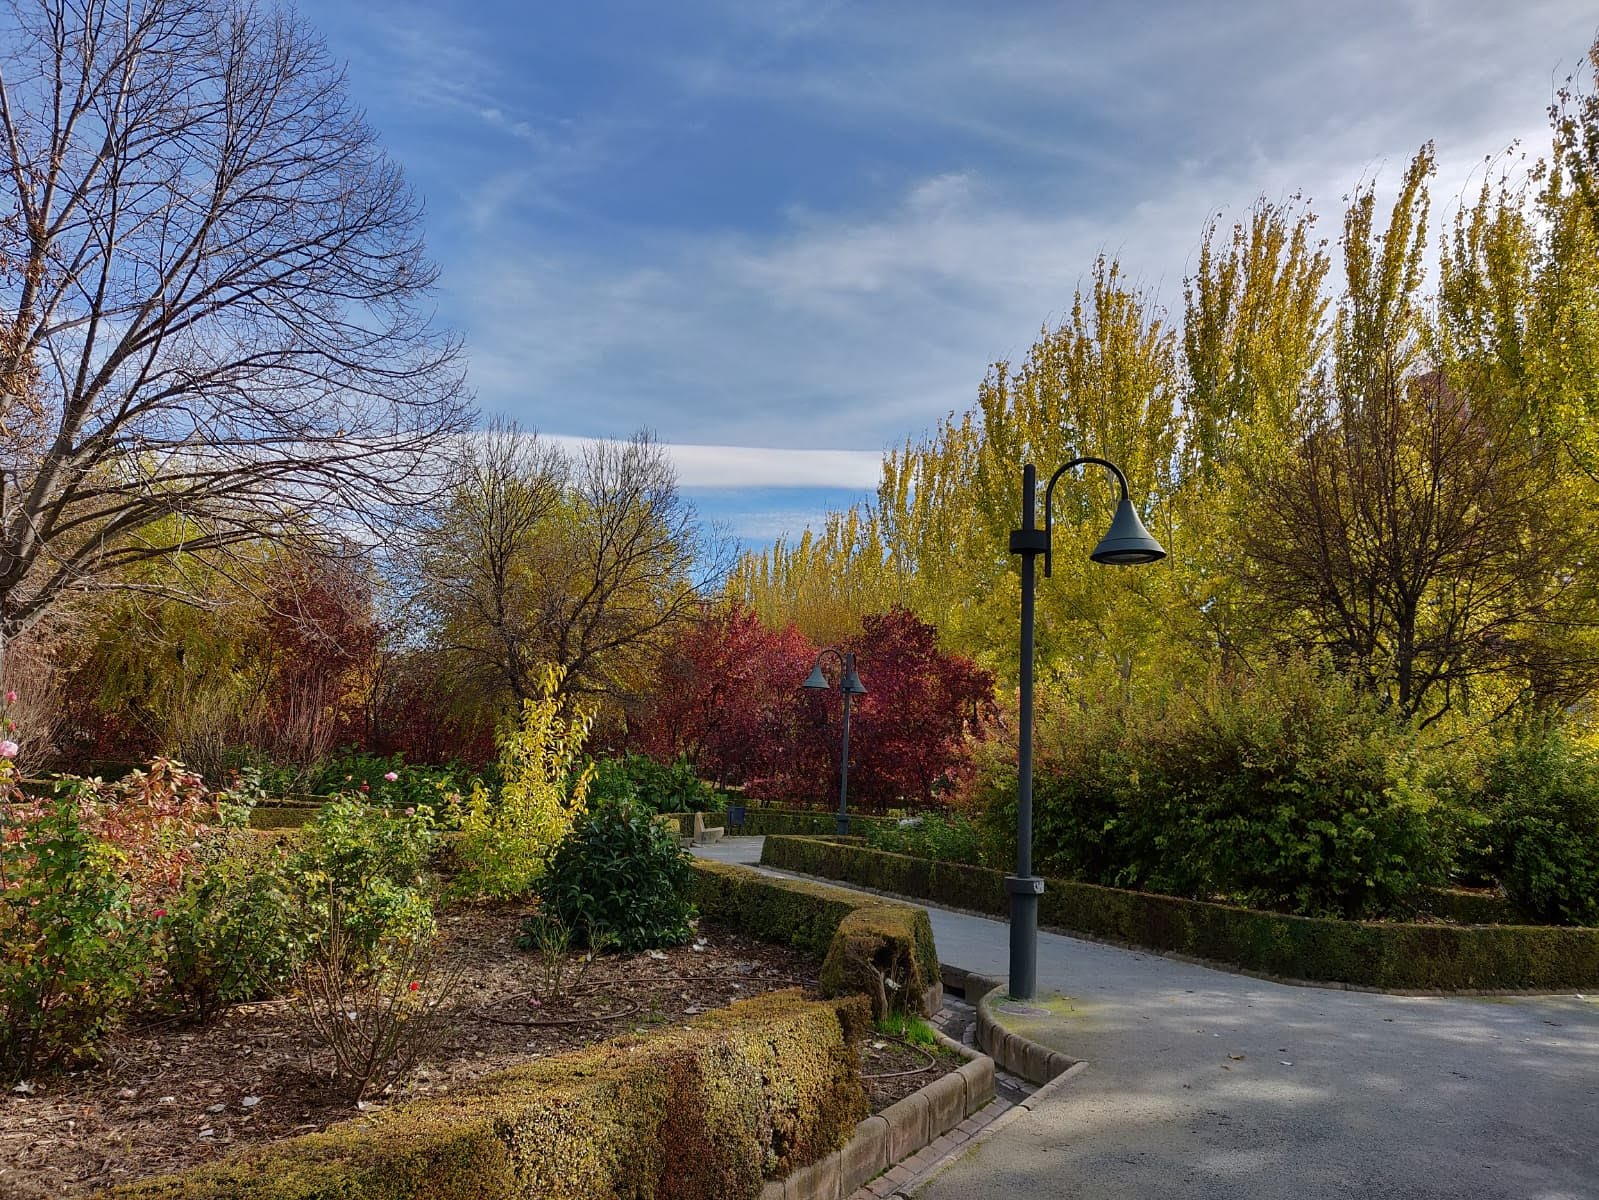
\includegraphics[width=0.5\textwidth]{Fotos/texturas.jpg}
		\end{figure}	
\end{itemize}

\begin{table}[H]
\centering
\begin{tabular}{|c|c|c|c|}
\hline
\diagbox[width=15em]{\textit{Códec}/Formato}{\\Información} & Tamaño & Valoración & Ranking \\
\hline
\textsc{bmp} &  &  &  \\ \hline
\textsc{tiff} sin compresión &  &  &  \\ \hline
\textsc{tiff} con deflación &  &  &  \\ \hline
\textsc{gif} &  &  &  \\ \hline
\textsc{jpeg} con calidad :100 &  &  &  \\ \hline
\textsc{jpeg} con calidad :50 &  &  &  \\ \hline
\textsc{jpeg} con calidad :5 &  &  &  \\ \hline
\textsc{png} &  &  &  \\ \hline
\end{tabular}
\caption{Imagen poco cromática}
\label{tab:my-table}
\end{table}


\subsection{Imagen con texto}

Esta primera imagen, mostrada debajo, utilizaremos una imagen tomada de un manga, los cuales son impresos en escala de grises.

\begin{itemize}
	\item Formato original: \textsc{.bmp}
	\item Tipo de imagen: texto
	\item Imagen:
		\begin{figure}[H]
		\centering
			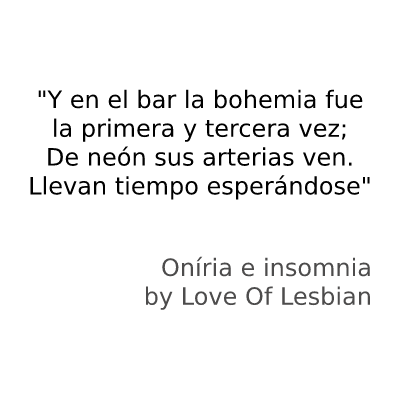
\includegraphics[width=0.5\textwidth]{Fotos/texto.png}
		\end{figure}	
\end{itemize}

\begin{table}[H]
\centering
\begin{tabular}{|c|c|c|c|}
\hline
\diagbox[width=15em]{\textit{Códec}/Formato}{\\Información} & Tamaño & Valoración & Ranking \\
\hline
\textsc{bmp} &  &  &  \\ \hline
\textsc{tiff} sin compresión &  &  &  \\ \hline
\textsc{tiff} con deflación &  &  &  \\ \hline
\textsc{gif} &  &  &  \\ \hline
\textsc{jpeg} con calidad :100 &  &  &  \\ \hline
\textsc{jpeg} con calidad :50 &  &  &  \\ \hline
\textsc{jpeg} con calidad :5 &  &  &  \\ \hline
\textsc{png} &  &  &  \\ \hline
\end{tabular}
\caption{Imagen poco cromática}
\label{tab:my-table}
\end{table}


\subsection{Imagen gráfica}

Esta primera imagen, mostrada debajo, utilizaremos una imagen tomada de un manga, los cuales son impresos en escala de grises.

\begin{itemize}
	\item Formato original: \textsc{.bmp}
	\item Tipo de imagen: gráfica
	\item Imagen:
		\begin{figure}[H]
		\centering
			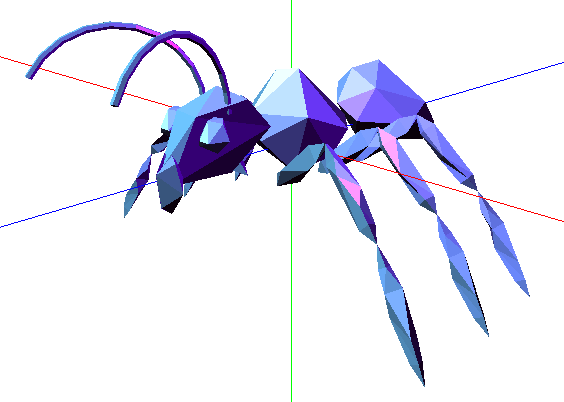
\includegraphics[width=0.5\textwidth]{Fotos/graficos.png}
		\end{figure}	
\end{itemize}

\begin{table}[H]
\centering
\begin{tabular}{|c|c|c|c|}
\hline
\diagbox[width=15em]{\textit{Códec}/Formato}{\\Información} & Tamaño & Valoración & Ranking \\
\hline
\textsc{bmp} &  &  &  \\ \hline
\textsc{tiff} sin compresión &  &  &  \\ \hline
\textsc{tiff} con deflación &  &  &  \\ \hline
\textsc{gif} &  &  &  \\ \hline
\textsc{jpeg} con calidad :100 &  &  &  \\ \hline
\textsc{jpeg} con calidad :50 &  &  &  \\ \hline
\textsc{jpeg} con calidad :5 &  &  &  \\ \hline
\textsc{png} &  &  &  \\ \hline
\end{tabular}
\caption{Imagen poco cromática}
\label{tab:my-table}
\end{table}


\subsection{Conclusiones}

Como se ha observado en las tablas anteriores, la resolución de 8 bits siempre es muy mala, mala o regular en el mejor caso, ya que en todas las pistas de audio se escucha un zumbido muy molesto que hace que con esta resolución pierda mucha calidad y no sea agradable escuchar la pista de audio. Aunque el resto de la melodía y las voces se escuchen bien, ese ruido resulta muy desagradable y, aunque se mantenga la calidad del resto del audio, se hace imposible poner una buena calificación.\\

Además, en cada pista de las tres diferentes, las tablas varían, especialmente la grabación de voz con respecto a las otras dos, tal vez debido a la calidad original del propio audio, lo que nos lleva a que la grabación, que originalmente estaba comprimida con el códec \textsc{aac}, tenga mucha diferencia con respecto a los audios que no tenían ningún tipo de compresión.


\section{Software utilizado}

Para poder cambiar los parámetros de digitalización y para poder cambiar los distintos \textit{códecs}, se ha utilizado \textbf{\textit{SoundConverter}}, que permite modificar y generar pistas de audio como se desee, con distintas frecuencias de muestreo (hay más frecuencias de las que se han utilizado en las tablas del apartado de parámetros de digitalización).\\

\begin{itemize}
	\item \textcolor{blue}{\url{https://soundconverter.org/}}
\end{itemize}

\section{Bibliografía}

\begin{itemize}
	\item Transparencias de teoría de Sistemas Multimedia: el sonido
	\item \footnotesize{\textcolor{blue}{\url{https://www.maketecheasier.com/convert-flac-to-mp3-easily-with-soundconverter/}}}
\end{itemize}

\end{document}